\chapter{Introdução}\label{introducao}

\chapter{Fundamentação Teórica}\label{fundamentacao}
% Som
% pressao sonora
% potencia
% calculo potencia anecoica
% calculo potencia reverberante

\chapter{Descrição do Experimento}\label{descricao}
% instrumentos de medicao
% Medição de pressão sonora na câmara semi-anecoica
% Medição de pressão sonora na câmara reverberante

% codigo

\chapter{Resultados}\label{resultados}
% grafico semianecoica
% grafico reverberante


\chapter{Conclusões}\label{conclusoes}



  
   %   \begin{figure}[h!]
   %     \centering
    %    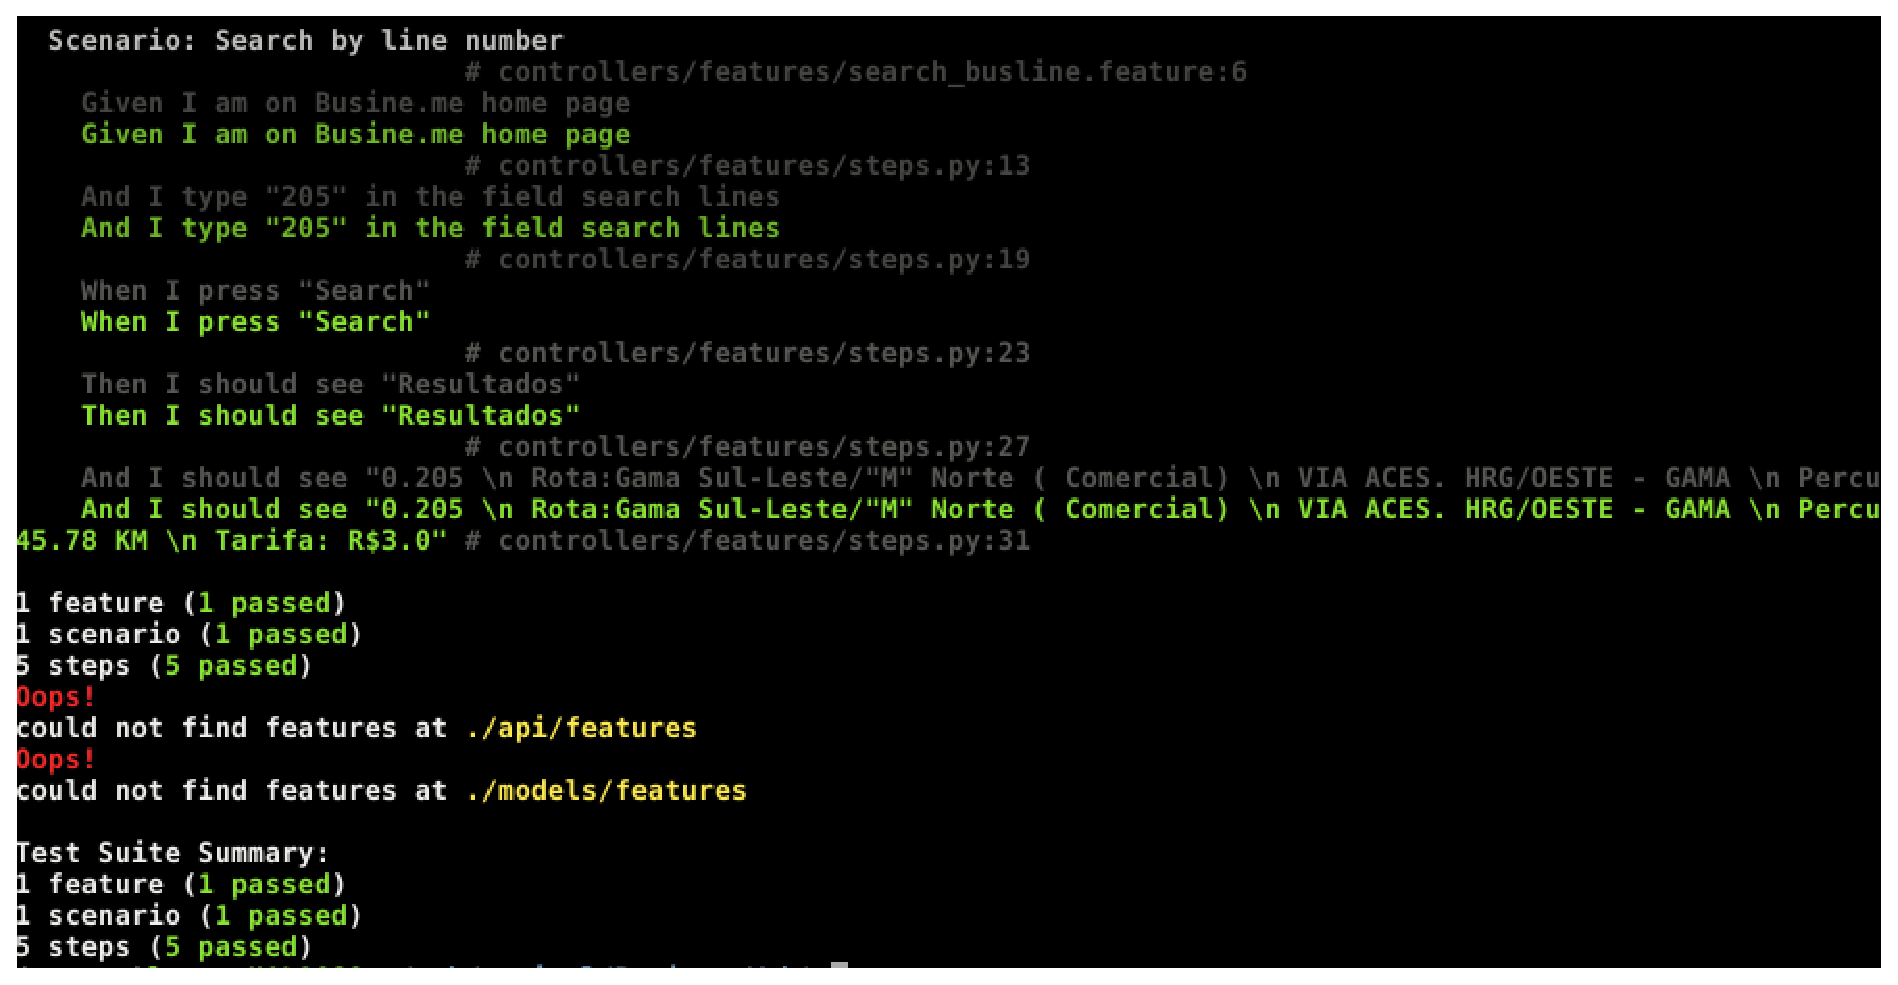
\includegraphics[width=0.9\textwidth]{figuras/results_2.eps}
     %   \caption{Resultado dos testes usando o splinter ao rodar o comando
      %  python manage.py harvest}
    %\end{figure}


